\documentclass[12pt]{article}
\usepackage{float}
\usepackage{graphicx}
\usepackage{fontspec}
\usepackage{titlesec}
\usepackage{setspace}
\usepackage[style=numeric,backend=biber,sorting=none]{biblatex}
\usepackage[a4paper, total={6in, 8in}, margin=0.5in]{geometry}
\addbibresource{ref.bib}

%%%%%%%% FORMAT
\singlespacing
\setmainfont{Arial}

\titleformat*{\section}{\normalsize\bfseries}
\titleformat*{\subsection}{\normalsize\bfseries}

\pagenumbering{gobble} % Suppress page number

% \titlespacing\section{0pt}{12pt plus 4pt minus 2pt}{0pt plus 2pt minus 2pt}
% \titlespacing\subsection{0pt}{12pt plus 4pt minus 2pt}{0pt plus 2pt minus 2pt}
% \titlespacing\subsubsection{0pt}{12pt plus 4pt minus 2pt}{0pt plus 2pt minus 2pt}


\begin{document}
  
%%%%%%%%% TITLE  
\title{\large Are core Laboratory necessary for resarch? \vspace{-2em}}
% \author{\large Yujia Shi\vspace{-1em}}
\date{\vspace{-2.5em}}
\maketitle

%%%%%%%%% BODY TEXT
\section{INTROUDCTION}
The concept of core laboratory introduced in life science is driven by the emergence of expensive sequencing technologies. After the completion of the Human Genome Project, we are moving forward to the era of post-genomic. Several leading research institutions have noticed that life science study greatly relies on specific technologies and services, without the support from this rapid development of technologies, it is impossible to make any significant breakthrough in research. Therefore, it's crunch time to begin focus on establishing a laboratory in which it will make every endeavor to warrant access to the latest technologies platform that can not afford and master by an individual researcher, particularly for newly established labs.
\medskip

\section{IMPORTANT ROLE OF CORE LABORATORY}
Core laboratory is playing an important role across branches of the science field, including mathematic, computer science, chemistry as well as biomedical science. The mission of the core laboratory is to provide expertise experience and access to cutting-edge equipment, for example, giving advice on which kind of equipment can be applied to your project or giving training sessions to make users equipped with the knowledge to use the equipment properly. All of these will enable researchers to implement their project in a time-efficient and cost-effective way.\medskip

Take our school for example, there are 7 core laboratories located on different floors of our school, i.e., Microscopy and Imaging core, Bio-fabrication Core, Histology Core, Flow Cytometry Core, Proteomics Core, Macromolecular and Microarray Core, and Animal Holding Core, serving as an important component with different functions for countless ongoing project, for example, core lab personnel may involved in the early planning stage of the project, to help with data analysis, figure preparation, and on-site technical assistance. These core facilities are responsible to guide both internal and external users to implement and design their research out with multiple technologies, the core lab staffs will host a training session before giving authority to the user of manipulating pieces of equipment and engaging in any laboratory activities. For those never get in touch with these instruments in the past time, the training session is designed for them to have the technical knowledge, basic understanding of tools used that may improve his or her daily laboratory safety operation and accelerate the whole process of the research.
\medskip

Furthermore, the additional value of the core laboratory is that fosters a collaborative research environment by holding up a regular seminar session. Through attending the seminars, not only can get to know more about the state-of-the-art equipment but also scientists from different background and disciplines can exchange and integrate their research idea and expertise with others, it is helpful to receive diverse experiences and skills from people who are at a similar or non-identical background when you are struggling with complex and important problems, in other words, a pipeline or a solution applied to one project may later use for another user with different problems. Thus, it is unquestionable that participating in the seminar will allow us to keep up with the latest technologies as well as forming a collaboration with others, and thereby making progress on their respective research. 

\section{THE FOUR PILLARS}
As we mentioned above, the core laboratory is an indispensable component in the research ecosystem. To build up a maintainable and productive core laboratory, after long deliberation, people coming out four pillars of the model to ensure the core facility can operate smoothly, in turn helping researchers from any institution to speed up their involved project.

\subsection{CORE PERSONNEL}
The core staff is the fundamental of the core Laboratory, with their continuous dedication and provide technical professional skills, a scientist from different departments or institutes can knick off their research more efficiently and effectively by accessing the sophisticated and expensive of technologies. Core facility staff usually falls into two categories, one is exempt staff, the other is the nonexempt staff. Exempt staff including core scientists and core managers are taking up the duty of serving as an expert in the domain field to providing their practical technical experience to meet researchers' needs. Both core scientists and managers are hired with a strong research background and are required to have advanced training in the area relating to the core facility. For nonexempt comprised of core research technician and research technician lead. Comparing to exempt staff, they are internally focused, being a technical expert with abundant hands-on experience in a core lab facility and responsible for data collection. In short, core facility staff is support and independent unit not belong to any of the research groups in the research ecosystem, they are larger enough to giving out professional assistance to the needs of users. Besides, the cores lab must be neutral, instead of choosing the demanding project or users based on their own preference or specified criteria, they need to assess each project on the objective perspective and the fundamental of technical workability, in order making the research institutes attain the highest level of progress in future of research.


\subsection{CORE SPACE}
Core laboratory is a self-reliant space, where researchers can reach state-of-the-art equipment and services. According to the space requirement, the core laboratory can be classified into two types: instrument-focused and service-focused facilities. For instrument-focused facilities including microfabrication, NMR, microscopy, medical imaging, which requires larger space to make sure the training session can be carried out smoothly, the instrument can be properly stored as well as avoid contiguous workspace bothering with each other. In contrast to instrument-focused facilities,service-focused demands relatively small space but at the expense of a higher personnel cost. Instead of using instruments, the space for service-focused is to lend a helping hand or assistance with data preparation, analysis, or even manuscript writing. The results giving back to users mostly are data files or physical items.

\subsection{INSTITUTIONAL INVESTMENT}
To keep up with the growing rate of science and technologies, university and research institutions both should have a detailed arrangement for core laboratory of its groundwork, staff and building up collaboration with other institutions, all of which is to adapt to the rapid change of research environment as well as meet the demand from researchers.
(i) Equipment Support 
More expenditure will be required for equipment investment, to help the core laboratory to keep their service and instruments up-to-date. The investment plan comprised of acquiring, upgrading, and maintaining instruments, each is equally important to each other. Besides, when more new equipment is introduced into the core laboratory, the more Service-oriented expert scientists who are equipped with technical professionals will be hired to handle these issues.
(ii) Operation Support 
The utilization rate of the core laboratory by researchers is also the key factor influence the sustainability of core facilities. As the operation of the core laboratory is based on fee-for-service, without sufficient support from the users, subsidizing from research institutions will be vital.

\subsection{INSTITUTIONAL EVALUATION}
People are not enjoyed being evaluated, they believe the evaluation activity is time-consuming and usually coming out with useless conclusions. Nevertheless, the evaluation process is one of the important pillars to ensure the core laboratory is operating in productiveness and an effective manner. For the core director, the assessment process provides them important information when making critical decisions and investments about whether to continue or discontinue supporting the area or not. Without the evaluation, it is impossible to build up or improve the core facility that is more effective and tailored to research's demand and expectations. There are a great number of strategy can be used to assess many aspects of core laboratory, for example, Goals-Based Evaluation, Process-Based Evaluations, and Outcomes-Based Evaluation, and so on. The following three processes are relatively common within this evaluation approach. One is annual reports, another is annual users, the other is program review. (i) Annual Report:
The assessment of the annual report is available in a spider diagram with eight different aspects: general management, research and technical staff, financial management, customer base and satisfaction, customer publications and grants, educational and outreach activities, communication of services, and self-assessment. The advantage of the annual reports allows the core laboratory to take measures for improvement and development, corresponding to the reflected evaluation. (ii) Annual Survey: The procedure of carrying out an annual survey is to sent out the questionnaire to external, internal as well as potential users. The survey composes of vast massive information on user behavior and experience in the past few years, all of which can serve as critical criteria, guiding the future striving direction.(iii) Program review: Even though annual reports and annual surveys are efficient tools for assessment, however, sometimes they are incapable of solving the elementary issues in the core laboratory, for example, controversial among faculty advisors or duplicated service and so on. Perform program review is aiming to address the basement problems by inviting externals experts to conduct an assessment and suggestion.


\begin{figure}[H]
    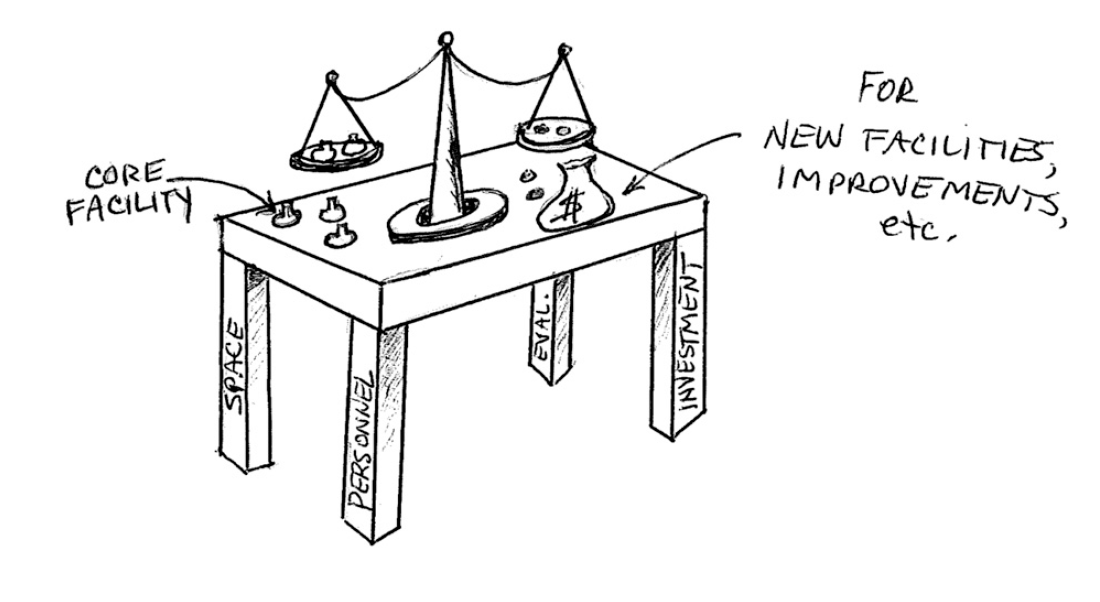
\includegraphics[width= 1 \columnwidth]{/Users/yu-pinglin/Desktop/Essay/6002_corelab.png}
    \centering
    \caption{Changes in the cost of sequencing over time}
\end{figure}


\section{CONCLUSIONS}
There is no doubt that interdisciplinary research as well as the multi-domain scientific progress can obviously benefit from the contribution of the core laboratory by promoting the opportunity for collaboration. However, there are still some factors that impede them to exert full potentials. To leveraging the full potential of core laboratory, and ensure we are on the path toward developing financial sustainability of core laboratory, by operating the core laboratory on a fee-on-service framework, which is not sufficient enough only supported by operating the core laboratory on the fee-on-service framework.As modern technologies are evolving in an exponential phase, customer revenues are unlikely to cover its operating costs
enough to support the core laboratory to keep up watching state-of-art technologies and equipment, and therefore, it will need significant investment from the corresponding institution.Only with steady growth in use revenue and constant support from institutions could core laboratory keep making satisfactory progress in the research ecosystem.


\emergencystretch=1em
\printbibliography[title=Reference]

\end{document}




